\documentclass[a4paper,12pt,twoside]{hmcpset}
\usepackage[utf8]{inputenc}
\usepackage[english]{babel}
\usepackage{fancyhdr}
\usepackage[margin=1in]{geometry}
\usepackage{graphicx}
\usepackage{amsmath}
\usepackage{mathtools}
\usepackage[mathscr]{euscript}
%\newcommand*{\ms}[1]{\ensuremath{\mathscr{#1}}}
\usepackage{lmodern} % math, rm, ss, tt
\usepackage[T1]{fontenc} 

\pagestyle{fancy}
\fancyhf{}
\rhead{Spring 2019}
\chead{Section 4}
\lhead{\vspace{3mm} Math 147 Topology}
\rfoot{Page \thepage}
\linespread{1.3}
 
\renewcommand{\headrulewidth}{2pt}
\renewcommand{\footrulewidth}{2pt} 

\graphicspath{ {./figures_theorems_sect_4/} } 

% info for header block in upper right hand corner
\begin{document}
\section*{Chapter 4\\\\
                    Bases, Subspaces, Prodcuts: Creating New Spaces} 
\begin{problem}[Theorem 4.1] Let $(X, \mathscr{T})$ be a topological
    space and $\mathscr{B}$ be a collection of subsets of $X$. Then
    $\mathscr{B}$ is a basis for $\mathscr{T}$ if and only if:\\
    1. $\mathscr{B} \subset \mathscr{T}$\\
    2. for each set $U$ in $\mathscr{T}$ and point $p$ in $U$ there is
    a set $V$ in $\mathscr{B}$ such that $p \in V \subset U$
\end{problem}

\begin{proof}
    First we prove the forward direction. Suppose we have a set
    $\mathscr{B}$ such that $\mathscr{B} \subset \mathscr{T}$,
    and for every open set $U \in \mathscr{T}$ and point $p$ in $U$
    there is a set $V$ in $\mathscr{B}$ such that $p \in V \subset U.$
    \\
    Then let $A$ be an open set of $X$. For all $a \in A$, there exists an
    open set $V_a \in \mathscr{B}$ such that $a \in V_a \subset A$.
    Then observe that 
    \[
      \bigcup\limits_{a \in A} V_a = A.
    \]
    Thus we see that every open set in $X$ is the union of elements of
    $\mathscr{B}$, so $\mathscr{B}$ is a basis for $X$.
    \\
    \\
    Now we prove the other direction, and suppose $\mathscr{B}$ is a
    basis for $X$. First observe that $\mathscr{B}
    \subset \mathscr{T}$ because this is part of the definition of a
    basis, so this proves (1). Now let $U \in \mathscr{T}$. Then 
    \[
      \bigcup_{B \in \mathscr{B}'} B = U
    \]
    for some subset $\mathscr{B}'$ of $\mathscr{B}$.
    Thus for any $p \in U$, there must exist at least one
    $B\in \mathscr{B}'$ such that $p \in
    B$ and by construction $B \subset U$. Therefore, we have that for 
    each set $U$ in $\mathscr{T}$ and point $p$ in $U$ there is
    a set $B$ in $\mathscr{B}$ such that $p \in B \subset U$, as desired.
\end{proof}

Ex: the set of length 1 intervals. This does not generate a topology
on $\mathbb{R}$ because intersections should be open but sometimes
they are intervals of length less than 1. \\
Another topology is the stick bubble topology. Open sets are balls
sitting in the upper half plane or an open ball containing a single
point on its circumference which is shared with the boundary of the
upper half plane. \\
\\
Ordered set topology: \\ 
\newpage
\noindent\rule{18cm}{1pt}
\textbf{Exercise 4.2}\\
1. Let $\mathscr{B}_1 = \{(a,b) \subset \mathbb{R} : a, b \in
\mathbb{Q}\}$. Show that $\mathscr{B}_1$ is a basis for the standard
topology on $\mathbb{R}.$\\
2. Let $\mathscr{B}_2 = \{(a,b) \cup (c,d) \subset \mathbb{R} : a < b
< c < d \text{ are distinct irrational numbers.}\}$ Show that
$\mathscr{B}_2$ is also a basis for the standard topology on
$\mathbb{R}.$ 
\\\noindent\rule{18cm}{1pt}\\

\begin{solution}
    1. We can do this using Theorem 4.1. Observe firstly that $\mathscr{B}_1 \subset
\mathscr{T}_\text{std}$. Now consider an arbitrary open set $U$ in 
$\mathbb{R}$. By definition, for any $p \in U$ there exists an open
ball $B(p, \epsilon(p))$ such that $p \in B(p, \epsilon(p)) \subset
U$. 
Since
the rationals are dense in $\mathbb{R}$, for any $p \in U$ 
there must exist a rationals
$a/b$ and $c/d$ such that 
\[
    p - \epsilon(p) < a/b< p < c/d < p +
\epsilon(p).
\] 
Thus $(a/b, c/d) \in \mathscr{B}_1$ and 
$p \in (a/b, c/d) \subset B(p, \epsilon) \subset
U$. 
This
proves (2) of the theorem, so $\mathscr{B}_1$ is a
basis for the standard topology on $\mathbb{R}$. \\
\\
2. We can do this using Theorem 4.1. Observe firstly that $\mathscr{B}_1 \subset
\mathscr{T}_\text{std}$. Now consider an arbitrary open set $U$ in 
$\mathbb{R}$. By definition, for any $p \in U$ there exists an open
ball $B(p, \epsilon(p))$ such that $p \in B(p, \epsilon(p)) \subset
U$. 
Since
the irrationals are dense in $\mathbb{R}$, for any $p \in U$ 
there must exist a rationals
$a, b, c$ and $d$ such that 
\[
    p - \epsilon(p) < a< p < b < c < d < p +
\epsilon(p).
\]
Thus $(a, b) \cup (c, d) \in \mathscr{B}_2$ and 
$p \in (a, b) \cup (c, d) \subset B(p, \epsilon) \subset
U$. 
This
proves (2) of the theorem, so $\mathscr{B}_2$ is a
basis for the standard topology on $\mathbb{R}$.
\end{solution}

\begin{problem}[Theorem 4.3] Suppose $X$ is a set and $\mathscr{B}$ is
    a collection of subsets of $X$. Then $\mathscr{B}$ is a basis for
    some topology on $X$ if and only if:\\
    1. Each point of $X$ is in some element $\mathscr{B}$\\
    2. if $U$ and $V$ are sets in $\mathscr{B}$ and $p$ is a point in
    $U \cap V$, there is a set $W$ of $\mathscr{B}$ such that $p \in W
    \subset (U \cap V)$.
\end{problem}
    
\begin{figure}[h]
    \centering
    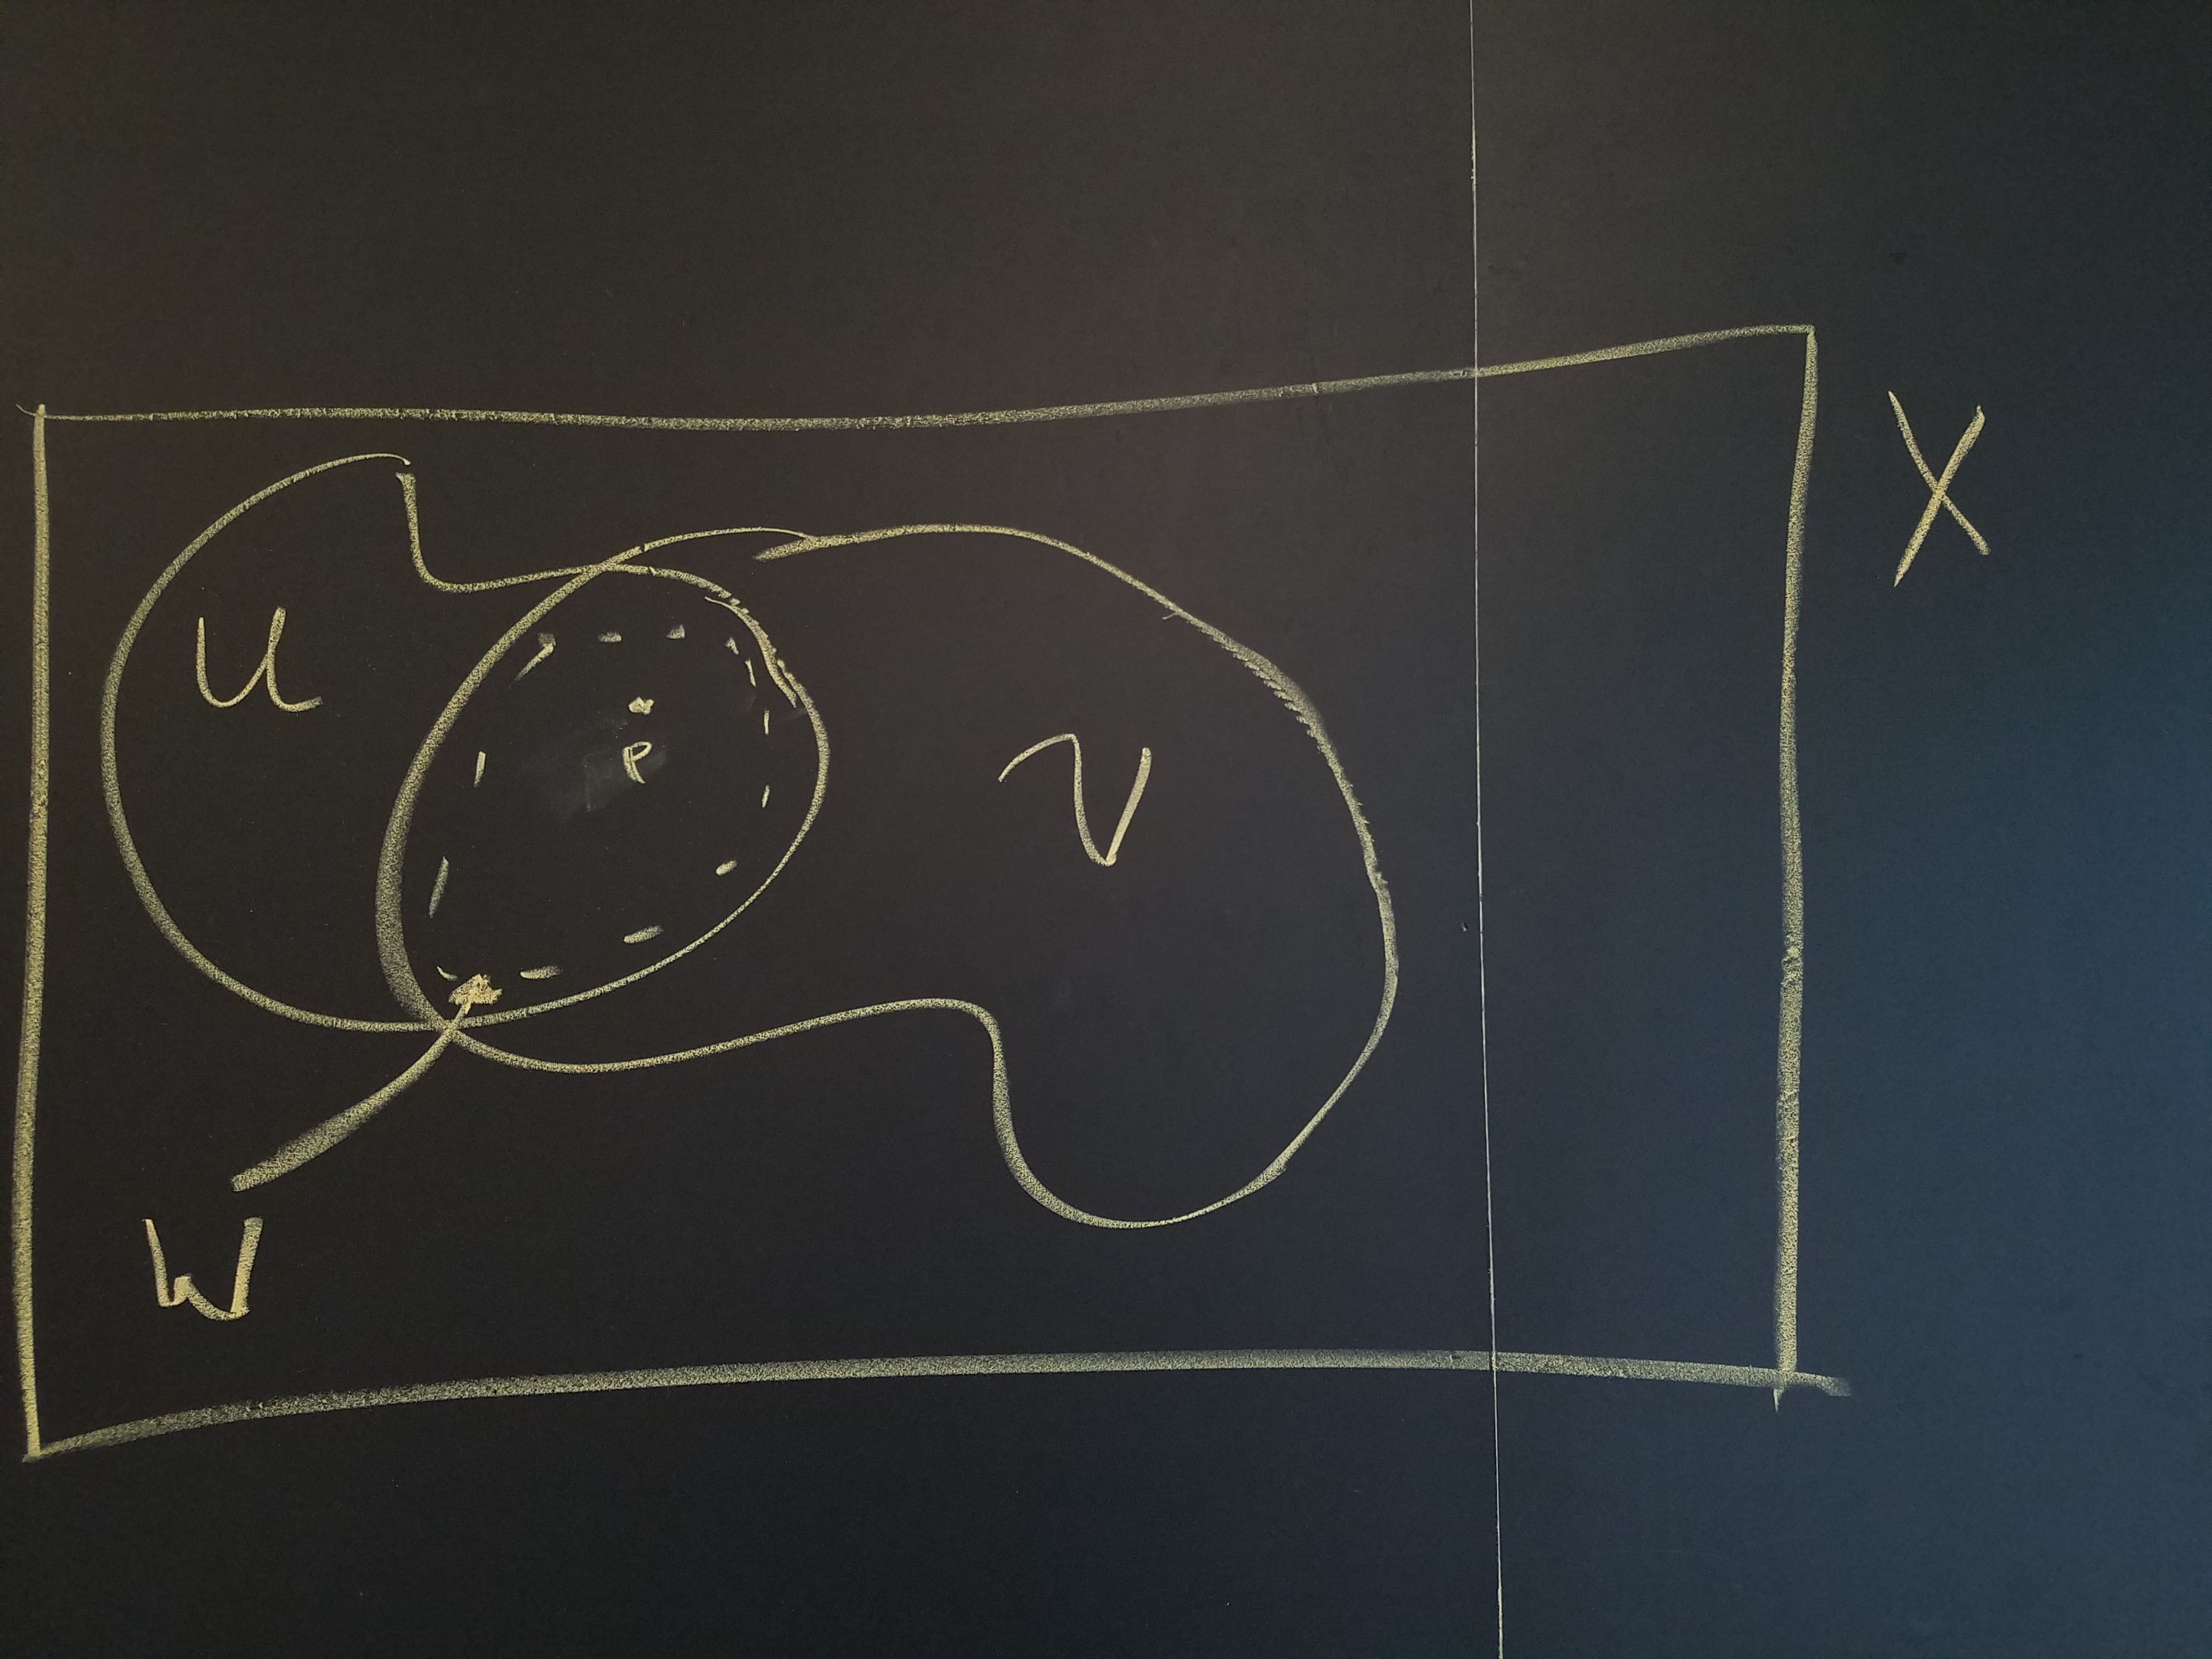
\includegraphics[width=0.7\textwidth]{sketch_theorem_4_3.jpg}
    \caption{Here we have sketched the conditions (1) and (2), where
    $X$ is the whole space, $U, V \in \mathscr{B}$ and $W \in (U \cap
    V)$.}
\end{figure}

\begin{proof}
    First we'll prove the forward direction. 
    Suppose that $\mathscr{B}$ is a basis for some topology
    $\mathscr{T}$. Since $X \in \mathscr{T}$, we know by Theorem 4.1
    that for every $p \in X$ there exists a $B \in \mathscr{B}$ such
    that 
    \[
    p \in \mathscr{B} \subset X.    
    \]
    Thus this proves (1).
    Next observe that if $U, V \in \mathscr{B}$, then $U, V \in 
    \mathscr{T}$. Therefore, $U \cap V \in \mathscr{T}$ is an open set
    in $X$. By Theorem 4.1, for any $p \in U \cap V$, there must exist
    a $W \in \mathscr{B}$ sucht that 
    \[
      p \in W \subset U \cap V.  
    \]
    This proves (2) which finishes the proof in this direction.
    
    
    
    Suppose that (1) and (2)
    are true. Then consider the set of all possible unions of elements
    of $\mathscr{B} = \{B_\alpha\}_{\alpha \in \lambda}$, namely the
    set 
    $$
    \mathscr{T} = \{\bigcup\limits_{\alpha \in \lambda'} B_{\alpha} :
     \lambda'\subset \lambda\}.
    $$ 
    We can now verify the properties that this is a topology.
    \begin{itemize}
        \item[1.] Observe that $\emptyset \in \mathscr{T}$
        if we take an empty union of objects. 

        \item[2.] $X
        \in \mathscr{T}$ by condition (1).

        \item[3.] Observe that arbitrary unions of
        elements of $\mathscr{B}$ are within $\mathscr{T}$, since that is
        by definition how we constructed $\mathscr{T}$.

        \item[4.] By condition (2) if $U, V \in \mathscr{B}$ 
        then there exsits
        a $W$ such that $W \in \mathscr{B}$ and $p \in W \subset (U \cap
        V)$. Thus observe that  
        \[
          U \cap V = \bigcup\limits_{p \in U \cap V} W_p 
        \]  
        where $W_p \in \mathscr{B}$ such that $p \in W_p \subset U
        \cap V$. By our definition of our topology, $U \cap V$ must be
        an open set. Therefore, finite interesections of open sets are open.

    \end{itemize}
    Thus we have shown that conditions (1) and (2) generate a
    topology, which completes the proof.

\end{proof}

\begin{exercise}[Exercise 4.4] Show that the basis proposed above (all sets of
the form $[a,b) = \{x \in \mathbb{R} : a \le x < b\}$) for the lower
limit topology is in fact a basis.
\end{exercise}

\begin{solution}
    We can show that this is a basis by using Theorem 4.3. Observe that
for any point $p \in \mathbb{R}$, there exists $a,b \in \mathbb{R}$
such that $a \le p < b$. Thus every point in $\mathbb{R}$ is in some
element of our basis. Next, let $c < d < e < f$ and consider $U = [c,
d]$ and $V = [e ,f]$. Then $U \cap V = \emptyset \in
\mathbb{R}_{\text{LL}}$.
\\
Next, let $c < d$ and $e < d < f$, and consider
the sets $U = [c, d)$ and $V = [e, f)$. Then there is a point $p \in
(U \cap V)$. Observe that if $\epsilon < p - e$ then the set $ 
p \in [p - \epsilon, f) \subset U \cap V$ and $[p - \epsilon, f)$ 
is a member of our
basis. Thus we have that sets of the form $[a, b)$ form a basis for
the lower limit topology. 

\end{solution}


\begin{problem}[Theorem 4.5] Every open set in $\mathbb{R}_\text{std}$
    is an open set in $\mathbb{R}_\text{LL}$, but not vice versa.
\end{problem}

\begin{proof}
    Consider an open set $B(p, \epsilon)$ in $\mathbb{R}_\text{std}$
    about a point $p$ of radius $\epsilon > 0$, which is really just
    an interval $(p - \epsilon, p + \epsilon)$. Then consider the
    sequence of open sets $\mathbb{R}_\text{LL}$:
    $$
    \left\{\left[p - \epsilon\left(1 - \frac{1}{2^n}\right), p + \epsilon\right) : n \in \mathbb{N}\right\}.
    $$
    Recall that an arbitrary union of open sets is open. Then
    $$
    \bigcup\limits_{n \in \mathbb{N}} 
    \left[p - \epsilon\left(1 - \frac{1}{2^n}\right), p + \epsilon\right)
    = (p - \epsilon, p + \epsilon)
    $$
    is an open set. Thus we have that open sets in
    $\mathbb{R}_\text{std}$ are open in $\mathbb{R}_\text{LL}$.
    However, it is obvious that open sets in $\mathbb{R}_\text{LL}$
    are not open in $\mathbb{R}_\text{std}$, because sets of the form
    $[a, b)$ are neither open or closed in $\mathbb{R}_\text{std}.$
    Thus this proves the theorem.
\end{proof}

\begin{exercise}[Exercise 4.6] Give an example of two topologies on
$\mathbb{R}$ such that neither is finer than the other, that is, the
two topologies are not comparable. 
\end{exercise}

\begin{solution}
    We can define an upper limit topology $\mathbb{R}_{\text{UL}}$ 
generated by basis sets 
$(a, b] = \{x \in \mathbb{R} | a < x \le b\}$. 
\\
\\
For each $x \in \mathbb{R} \in (x - \epsilon, x +
\epsilon] \in \mathbb{R}_{\text{UL}}$. In addition, observe that $(a,
b] \cap (c, d] = (b, c]$ if $b < c$ and $(a, d]$ if $b = c$ and
$\emptyset$ if $b > c$, all of which are basic open sets in the
topology. Thus by Theorem 4.3 this generates a topology. 
\\
\\
Now observe that neither of the topologies 
$\mathbb{R}_{\text{LL}}$ and $\mathbb{R}_{\text{UL}}$
are finer than the other, since neither is a subset of the other. Thus
these topologies on $\mathbb{R}$ are not comparable.

\end{solution}

\begin{exercise}[Exercise 4.7] Check that the collection of sets that we
specify as a basis in the double headed snake actually forms a basis
for the topology.
\end{exercise}

\begin{solution}
    We can verify this using theorem 4.3. Observe first that every point
in $\mathbb{R}_{+00}$ is contained within some set in the basis. Next,
let $U$ and $V$ be any two sets in the topology. Then if $U, V$ are of
the form $(0, b) \cup \{0'\}$, then their intersection will be of the
form $(0, a) \cup \{0'\}$ where $a \le b$ which is a set within our
basis. The argument applies again to if $U, V$ are both of the form
$(0, b) \cup \{0''\}$ or $(a, b)$. \\
\\
Next observe that if we intersect $U$ of the form $(0, b) \cup \{0'\}$
with $V$ of the form $(a, b)$ then the intersection is either empty,
or of the form $(a, b)$, which is a type of set contained in our
absis. If we intersct 
\\
Let $U$ be any set in $\mathbb{R}_{+00}$. Let $U = (a,b)$ where $a, b
\in \mathbb{R}$ and $a < b$. If $U$ does not contain $\{0'\}$ or
$\{0''\}$, then there exits numbers $c, d \in mathbb{R}$ such that $a
< c < d < b$. Then the set $(c, d)$ is in our basis and is a subset of
$U$.
\end{solution}


\begin{exercise}[Exercise 4.8] In the Double Headed Snake, show that every
point is a closed set; however, it is impossible to find disjoint open
sets $U$ and $V$ such that $\{0'\} \in U$ and $\{0''\} \in V$. 
\end{exercise}

\begin{solution}
Observe that the complement of every point is an interval of the line, for which we 
can represent as the union of basic open sets and therefore 
the complement of every point is open. Thus every point must be a
closed set. 
\\
\\
 Next, let $U$ be an open set
 containing $\{0'\}$ and $V$ an open set containing $\{0''\}$. Then by definition, 
 there must exist basic open sets $U_B$, $V_B$ such that $0' \in U_B \subset U$
 and $0'' \in V_B \subset V$. Since they are basic open sets containing the zeros 
 of the double headed snake, both are either of the form $(0, b) \cup \{0'\}$
 or $(0, b) \cup \{0''\}$, so that $U_B \cap V_B \ne \emptyset.$ Thus 
 we cannot find disjoint open sets $U$ and $V$ such that $\{0'\} \in U$ and $\{0''\} 
 \in V$.
\end{solution}

\noindent\rule{18cm}{1pt}
\begin{exercise}[Exercise 4.9]
1. In the topological space $\mathbb{R}_\text{har}$, what is the
closure of the set $H = \{1/n\}_{n \in \mathbb{N}}$?\\
2. In the topological space $\mathbb{R}_\text{har}$, what is the
closure of the sets $H^{-} = \{-1/n\}_{n \in \mathbb{N}}$?\\
3. Is it possible to find disjoint open sets $U, V$ in
$\mathbb{R}_\text{har}$ such that 0 $\in U$ and $H \subset V$?
\end{exercise}

\begin{solution}
    \begin{enumerate}
        \item There are no limit points to the set because all sets are of the
        form $(a,b)$ or $(a,b) - H$. Thus for any neighborhood about a point
        will always either not contain $H$ or it will exclude $H$, so by
        definition no point can be a limit point of $H$. 
    
        \item For $H^{-}$, the limit points just consists of the set $\{0\}$.
        This is any open set which contains 0 must contain points of the
        sequence $\{\frac{1}{n} | n \in \mathbb{N}\}$. The difference between
        this question and question (1.) is that in the first question, the
        points in the sequence were always excluded whenever they interesected
        any open set containing 0, whereas that's not the case here since we
        don't care about excluding the negative harmonics.
    
        \item For any open set $U$ containing 0, we must have that there exists
        an open set $U_0$ of 0 such that $0 \in V \subset U$. And since the
        basic open sets are $(a, b)$ or $(a, b) - H$, there must exist points
        to the right of 0 in the set $U$; otherwise, 0 would be a limit point.
        Because any open set containing $H$ must contain points arbitrarily
        close to 0, it is inevitable for $U$ and $V$ to intersect. This is
        because for any open set which contains $0$, say $(a, 0 + \epsilon)$
        for $\epsilon > 0$ and $a < 0$, there exsits an $n \in \mathbb{N}$
        such that $\frac{1}{n} < \epsilon$ and therefore any open set
        containing $H$ must contain this point and hence intersect with $(a, 0
        + \epsilon)$. Of course, any set of the form $(0 - \epsilon, b)$ for
        $b > 0$ will intersect with any set contanining $H$ by the same
        argument as before. Thus there does not exist disjoint open sets $U,
        V$ such that $0 \in U$ and $H \subset V$. 
    
    \end{enumerate}
\end{solution}

\begin{exercise}[Exercise 4.10]
    1. In $\mathbb{H}_\text{bub}$, what is the closure of the set of
rational on the $x$-axis?\\
\vspace{2mm}
\noindent
2. In $\mathbb{H}_\text{bub}$, which subsets of the $x$-axis are
closed?\\
\vspace{2mm}
\noindent
3. In $\mathbb{H}_\text{bub}$, let $A$ be a countable set on the
$x$-axis and $z$ a point on the $x$-axis not in $A$. Then there exist
open sets $U$ and $V$ such that $A \subset U$ and $z \in V$. (Do you
need the countability hypothesis on $A$?)\\
\vspace{2mm}
\noindent
4. In $\mathbb{H}_\text{bub}$, let $A$ and $B$ be countable sets on
the $x$-axis such that $A$ and $B$ are disjoint. Then there exists
open sets $U$ and $V$ such that $A \subset U$ and $B \subset V$.\\
\vspace{2mm}
\noindent
5. In $\mathbb{H}_\text{bub}$, let $A$ be the rational numbers and let
$B$ be the irrational numbers. Do there exist disjoint open sets $U$
and $V$ such that $A \subset U$ and $B \subset V$?
\end{exercise}

\begin{solution}
    \begin{enumerate}
        \item Suppose that a limit point was no a rational on the $x$-axis.
        Obviously such a point cannot be one which isn't on the $x$-axis since
        we could easily find an open set which contained that point but didn't
        intersect the $x$-axis. Thus our candidates for limit points for our
        set are reduced to irrationals on the $x$-axis. But observe that any
        open set which contains a rational doesn't necessarily contain an
        irrational. For example, any basic open set about a rational on the
        $x$-axis given by $(p, 0)$ does not contain an irrational. Thus the
        closure of the rationals is simply the rationals.
    
        \item Consider the set $\{(x,y) \in \mathbb{R}^2 | y > 0\}$; that is,
        everything but the $x$-axis. Observe that this set is simply the
        uncountable union of all possible basic open sets of the form $B((x,
        y), r)$ where $0 < r \le y$, so therefore this set must be open.
        Thererfore, its complement, the $x$-axis, must be closed. Furthermore,
        if we included in our uncountable union an arbitrary number of sticky
        bubbles of the form $B((x, y), r) \cup \{(x, 0\}$, which would form an
        open set, the complement would be a subset of the $x$-axis and it
        would be closed since the complement of open sets are closed. Thus all
        subsets of the $x$ axis are open.
    
        \item We argue that the countability hypothesis is not necessary. For any
        set $U$ containing $A$, $U$ must contain a set of sticky bubbles $B_x$
        of radius $r_x$ containing each point $x \in A$. Then if we can
        construct a sticky bubble of radius $r' < \max\{\sqrt{(z-x)^2 + r_x^2}
        - r_x^2\}$ about $z$, we see that $U$ and $V$ do not intersect. Thus
        there does exists disjoint open sets $U$ and $V$ such that $A \subset
        U$ and $z \in V$.
    
        \item Let $a \in A, b \in B$, and arbitrarily assign sticky balls
        $\{B_a\}$ each of radius $r_a > 0$ for each $a \in A.$ Then for each
        $b = (x_b, y_b)$, assign $b$ a sticky ball $B_b$ of radius $r$ such
        that $r < r'$ for all $$r' \in \{\sqrt{(x_a - x_b)^2 + r_a^2} - r_a^2
        | r_a \text{ is the radius of the sticky ball of point } (x_a, y_a)
        \in A\}.$$ If we do this for each point $b \in B$, and union the
        sticky balls $\{B_b\}$, we'll obtain an open set $V$ such that $B
        \subset V$. If we union all the sticky balls $B_a$, we'll again obtain
        an open set $U$ such that $A \subset U$, which proves the
        exercise.
        
        \item 
    \end{enumerate}    
\end{solution}

\begin{exercise}[Exercise 4.11]
    Check that the arithmetic progressions form a
basis of a topology on $\mathbb{Z}$.
\end{exercise}

\begin{solution}
    We can use Theorem 4.3 for this. Let the set of arithmetic progression
be $\mathscr{B}$ and let $q \in \mathbb{Z}$. Then
observe that $q \in \{p\cdot n : n \in \mathbb{Z}\} \in \mathscr{B}$.
Thus condition (1) of Theorem 4.3 is satisfied.
\\
\\ 
Now let $U, V \in \mathscr{B}$, and suppose $U = \{a_1n + b_1 : n \in
\mathbb{Z}\}$ and $V = \{a_2n + b_2: n \in \mathbb{Z}\}$. Suppose $U
\cap V$ is nonempty. Then $q \in U \cap V$ for some $q \in
\mathbb{Z}$. However, in order for $q$ to be in the intersection, we
must have tht $a_1$ and $a_2$ are coprime. If they are coprime, then
by Bezout's theorem that there exist integers $m_1, m_2$ such that 
$m_1n_1 + m_2n_2 = 1$. We then know by the Chinese
Remainder Theorem that $q = b_1 + (b_2 - b_1)m_1a_1$. Therefore, we
see that 
\[
    q \in \{ b_1 + (b_2 - b_1)na_1: n \in \mathbb{Z}\} \subset U \cap V.
\]
Since this is an arithmetic progression, this set lies in
$\mathscr{B}$. Therefore, we see that condition (3) of Theorem 4.3 is
satisfied, so that the arithmetic progressions do form a basis for a
topology on $\mathbb{Z}$.

\end{solution}

\begin{problem}[Theorem 4.12] 
    There are infinitely many primes. 
\end{problem}

\begin{proof}
    Let $p$ be prime and consider the set $p\mathbb{Z}$. Observe that 
    this is a closed set since it is the
    complement of the union of sets $p\mathbb{Z} + 1, \dots ,
    p\mathbb + (p -1)$ which are of the forms of basic open sets. 

    Now observe that nonempty open sets are always open. This is
    because every open set must contain a basic open set, which are by
    definition infinite sets.
    
    Thus suppose that there are infinitely many primes $p_1, p_2,
    \dots, p_n$. Then 
    \[
        \bigcup_{i = 1}^{n}p_i\mathbb{Z}
    \]
    is a closed set as it is the finite union of closed sets. However,
    note that 
    \[
        \left( \bigcup_{i = 1}^{n}p_i\mathbb{Z} \right)^c = \{-1, 1\}.
    \]
    This should be an open set, since $\bigcup_{i =
    1}^{n}p_i\mathbb{Z}$ is closed. But this is a contradiction since 
    $\{-1, 1\}$ is a finite set and hence cannot be open. Thus there
    must be an infinite number of primes.

\end{proof}


\begin{exercise}[Exercise 4.18]
Let $X$ be totally ordered by $<$. Let $\mathscr{S}$ be the collection
of sets of the following forms 
\[
\{x \in X | x < a\} \quad \text{ or } \quad \{x \in X | x > a\}
\]
for $a \in X$. Then $\mathscr{S}$ forms a subbasis for the order
topology on $X$. 
\end{exercise}

\begin{solution}
    We can prove this using Theorem 4.14. Observe that the first condition
    is satisfied because $\mathscr{S} \subset \mathscr{T}$. Next, let $p
    \in U \in \mathscr{T}$, and suppose that $U$ is of the form $\{x \in X
    | x < a\}$ or $\{x \in X | a < x\}$. Then observe that
    $U \in \mathscr{S}$ so that $\bigcap\limits_{n=1}^1 U \subset U$. Finally, suppose that
    $U$ is of the form $\{x \in X | a < x < b\}$. Then we can simply
    intersect the sets $S_1, S_2 \in \mathscr{S}$ where $S_1 = \{x \in X |
    a < x\}$ and $S_2 = \{x \in X | x < b\}$ to get that
    $\bigcap\limits_{n = 1}^2 S_n =
    \{x \in X | a < x < b\} \subset U$. Thus by condition (2) of Theorem
    4.14, we have that $\mathscr{S}$ must be a subbasis for the order
    topology.
\end{solution}

\begin{exercise}[Exercise 4.19]
Verify that the order topology on $\mathbb{R}$ with the usual $<$
order is the standard topology on $\mathbb{R}$. 
\end{exercise}

\begin{solution}
    Every set of the order topology is of the form $\{x \in \mathbb{R} | x < a\} \text{ or } \{x \in \mathbb{R} | a < x\}
\text{ or } \{x \in \mathbb{R} | a < x < b\}$ where $a, b \in
\mathbb{R}$. 
\\
\\
Consider a point $p$ in a set $U$ of the form of 
$\{x \in \mathbb{R} | x < a\} \text{ or } \{x \in \mathbb{R} | a <
x\}$. Then observe that $p \in B(p, |a - p|)$ is a ball containing $p$
inside $U$. By definition, these are therefore open sets in the
standard topology on $\mathbb{R}$. 
\\
\\
If instead $U$ is of the form $\{x \in \mathbb{R} | a < x < b\}$, then
for any $p \in U$ observe that $p \in B(p, \min\{p-a, b - p\})$, so that
$U$ must also be open in the standard topology on $\mathbb{R}$.
\\
\\
Finally observe that every open set in the standard topology on $\mathbb{R}$ is of the form of
a set in the order topology. This is because every open set in
$\mathbb{R}_\text{std}$ can be bounded from either one or both ends,
both possibilities which are captured by elements of the standard
topology on $\mathbb{R}$. Thus we can conclude that the order topology on $\mathbb{R}$ with the usual $<$
order is the standard topology on $\mathbb{R}$.
\end{solution}

\noindent\rule{18cm}{1pt}
\textbf{Exercise 4.20}\\
Draw pictures of various open sets in the lexigraphically ordered
square. 
\\\noindent\rule{18cm}{1pt}
\begin{figure}[h]
    \centering
    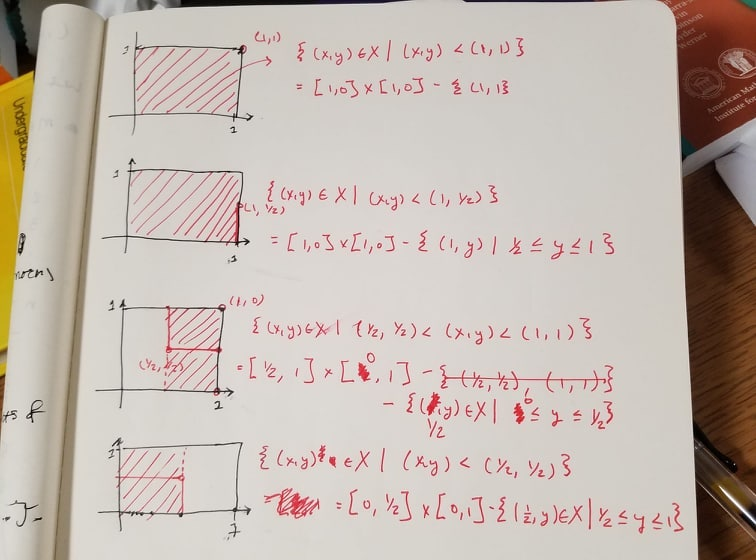
\includegraphics[width = 0.7\textwidth]{figures_theorems_sect_4/exercise_4_20.jpg}
    \caption{Here we consider three open sets $\{(x,y) \in X | (x, y)
    < 1\}$, $\{(x,y) \in X | (x, y) < (1, 1/2)\}$, $\{(x,y) \in X |
    (1/2, 1/2) < (x, y) <(1, 1) \}$ and $\{(x,y) \in X | (x, y) <
    (1/2, 1/2)\}$ and sketch their drawings. Since these are
    technically basis elements, we can also imagine unioning these
    sets around to obtain new open sets to imagine what the topology
    looks like.}
\end{figure}

\newpage
\begin{exercise}[4.21]
    In the lexigraphically ordered square find the closures of the
following subsets:
\begin{gather*}
    A = \left\{ \left(\frac{1}{n}, 0\right) | n \in \mathbb{N}\right\}\\
    B = \left\{ \left(1 - \frac{1}{n}, \frac{1}{2}\right) | n \in \mathbb{N}\right\}\\
    C = \left\{ \left(x,0\right) | 0 < x < 1 \right\}\\
    D = \left\{ \left(x, \frac{1}{2}\right) | 0 < x < 1\right\}\\
    E = \left\{ \left(\frac{1}{2}, y \right) | 0 < y < 1\right\}.
\end{gather*}
\end{exercise}

\begin{solution}
For set $A$, we argue that the set of limit points or the set $A$ is
simply the point $(0, 1)$. This is because for any open interval
containing $(0, 1)$, we must have the set wrap back around and include
a set of points $(x, 0)$ where $x > 0$ and is very small. Since the
sequence $\{\frac{1}{n}\}$ converges to 0, we see that an open set
$(0, 1)$ must include points of the sequence. Therefore (0,1) is a
limit point. \\
\\
For set $B$, observe that there are no limit points of $B$. The only
possible limit point would be $(1, \frac{1}{2})$, but we can find an
open set containing this point but no point of $B$. For example, the
set $\{(x,y) \in X | (1, 0) < (x, y)\}$ contains $(1, \frac{1}{2})$
but not any point of the set $B$. \\
\\
For the set $C$, we can see that the set of limit points will simply
be the set $\{(x, 1) \in X | 0 \le x < 1\} \cup \{(1, 0)\}$.
Basically, the the closure is the top and bottom lines of the unit
square, minus the two points $(0,0)$ and $(1,1 )$. \\
\\
The set $D$ has no limit points. This is because for any point $p =
(a, b)$, we can simply construct an open neighborhood about $p$ given
by 
$$\{(a,y) \in X | |y - b| < \min\{|b - \frac{1}{2}|, b - 1\} \}$$
which does not intersect the set if $b \ne \frac{1}{2}.$ In the case
where $b = \frac{1}{2}$, any neighborhood of the form 
$$U = \{(x, y) \in X | (a, 0) < (x, y) < (a, 1)\}$$ contains $p$, but
$(U - \{p\})\cap D = \emptyset.$ Therefore, there are no limit points
to the set so $\overline{D} = D$. \\
\\
For the set $E$, we see that the set of limit points is simply
$\{(\frac{1}{2}, 0), (\frac{1}{2}, 1)\}$. This is because any open set
containing either of these points must definitely contain points of
the set $E$. Thus the closure is $E \cup \{(\frac{1}{2}, 0),
(\frac{1}{2}, 1)\}$
\end{solution}


\begin{problem}[Theorem 4.25] Let $(X, \mathscr{T})$ be a topological
    space and $Y \subset X$. Then the collection of sets
    $\mathscr{T}_Y$ is in fact a topology on $Y$.
\end{problem}

\begin{proof}
We can show that $\mathscr{T}_Y$ is a topology by showing that it
satisfies the four criteria for the definition of a topology.
\begin{enumerate}
    \item Since $\mathscr{T}_Y = \{U | U = V \cap Y \text{ where } V \in
    \mathscr{T}\}$, we can take $V = \emptyset$ to observe that $\emptyset
    \in \mathscr{T}_Y.$

    \item Next, since $X \in \mathscr{T}$,
    we can take $V = X$ to observe that $X \cap Y = Y \in \mathscr{T}_Y.$

    \item Suppose $U, V \in \mathscr{T}_Y$ and consider $U \cap V$.
    Since $U = U' \cap Y$ and $V = V' \cap Y$ for some $U', V' \in
    \mathscr{T}$, we have that $U \cap V = (U' \cap Y) \cap (V' \cap Y) =
    (U' \cap V') \cap Y$. Since $(U' \cap V') \in \mathscr{T}$, then we
    know that $(U' \cap V') \cap Y = (U \cap V) \in \mathscr{T}_Y.$ Thus
    $\mathscr{T}_Y$ is closed under finite intersections.

    \item Now suppose $U_\alpha \in \mathscr{T}_Y$
    for all $\alpha \in \lambda$, where
    $\lambda$ is an arbitrary index. Then for each $\alpha$ there must exist a $V_\alpha \in
    \mathscr{T}$ such that $U_\alpha = V_\alpha \cap Y$. Thus
    $\bigcup\limits_{\alpha \in \lambda} U_\alpha = \bigcup\limits_{\alpha
    \in \lambda} (V_\alpha \cap Y) = \bigcup\limits_{\alpha \in \lambda}
    (V_\alpha) \cap Y $. Since $\bigcup\limits_{\alpha \in \lambda}
    V_\alpha \in \mathscr{T}$, we know that $\bigcup\limits_{\alpha
    \in \lambda} V_\alpha \cap Y \in \mathscr{T}_Y \implies
    \bigcup\limits_{\alpha \in \lambda} U_\alpha \in \mathscr{T}_Y.$ Thus we have that
    arbitrary unions of open sets are contained in $\mathscr{T}_Y.$
\end{enumerate}
Thus, we have that $\mathscr{T}_Y$ is a topology on $Y$.
\end{proof}

\begin{exercise}[Exercise 4.26]
Consider $Y = [0, 1)$ as a subspace for $\mathbb{R}_{\text{std}}$ In
$Y$, is the set $[1/2, 1)$ open, closed, neither or both? 
\end{exercise}

\begin{solution}
The set $[1/2, 1)$ is not open but is closed under this topology.
Firstly, there does not exist an element $V \in
\mathbb{R}_{\text{std}}$ such that $[1/2, 1) = V \cap Y$. Thus $[1/2, 1)$ is
not open in $\mathscr{T}_Y$. However, it is a closed set since it
contains its only limit point $1/2.$ This is because 
every open set which contains $1/2$ must
intersect with $[1/2, 1)$. Thus $[1/2, 1)$ is closed in the $Y$
subspace topology. 
\end{solution}

\begin{exercise}[Exercise 4.27]
Consider a subspace $Y$ of a topological space $X$. Is every subset $U
\subset Y$ that is open in $Y$ also open in $X$? 
\end{exercise}

\begin{solution}
Consider an open set $U \in \mathscr{T}_Y$. Then there exists a $V \in
\mathscr{T}_X$ such that $U = V \cap Y$. While the set $U$ is then
technically open in $\mathscr{T}_Y$, it is possible that $V \cap Y$ is
not an open set in $\mathscr{T}_X$, which would only happen in $Y \notin
\mathscr{T}_X.$ Thus we must have that $Y$ be open in order for the
above statement to be true. 
\end{solution}

\begin{problem}[Theorem 4.28] Let $(Y, \mathscr{T}_Y)$ be a subsapce
    of $(X, \mathscr{T})$. A subset $C \subset Y$ is closed in $(Y,
    \mathscr{T}_Y)$ if and only if there is a set $D \subset X$,
    closed in $(X, \mathscr{T})$, such that $C = D \cap Y$.
\end{problem}

\begin{proof}
    Let us first prove the forward direction. Suppose
    $D \subset X$ is closed in $(X, \mathscr{T})$ and let $C
    = D \cap Y$. Since $D$ is closed in $(X, \mathscr{T})$, we have
    that $X - D$ is open in the same topology. Now since $X - D \in
    \mathscr{T}$, observe that $(X - D) \cap Y \in (Y, \mathscr{T}_Y)$
    by definition. Since $(X - D) \cap Y$ is open in $(Y,
    \mathscr{T}_Y)$, the complement $Y - ((X - D)
    \cap Y)$ is closed. However, observe that $Y - ((X - D) \cap Y)= Y
    - (Y - D) = D \cap Y = C$, so that we have concluded that $C$ is a
    closed set. \\
    \\
    Now we prove the other direction. Suppose that $C$ is closed
    in $(Y, \mathscr{T}_Y)$. Since $C$ is closed, $Y - C$ is open
    in $(Y, \mathscr{T}_Y)$. Thus by definition, there exists a
    set $A \in \mathscr{T}_X$ such that $A \cap Y = Y - C$. Since
    $A$ is open, we know that $X - A$ is closed in $(X, \mathscr{T})$.
    Call this set $D$. Now observe that 
    $$D \cap Y = (X - A) \cap Y = (Y - A) \cap Y = C$$ because $A \cap Y
    = Y - C$. Thus we have found a set $D$ which closed in $(X,
    \mathscr{T})$ such that $C = D \cap Y$. Having proved both
    direction, this proves the theorem. 
\end{proof}

\begin{problem}[Corollary 4.29] Let $(Y, \mathscr{T}_Y)$ be a subspace
    $(X, \mathscr{T})$. A subset $C \subset Y$ is closed in $(Y,
    \mathscr{T}_Y)$ if and only if $\text{Cl}_X(C) \cap Y = C$
\end{problem}

\begin{proof}
    First we'll prove the forward direction. Suppose that
    $\text{Cl}_X(C) \cap Y = C$. Then let $p$ be a limit point of $C$
    in the topological space $(Y, \mathscr{T}_Y)$. Then for every set
    $U$ open in $(Y, \mathscr{T}_Y)$ which contains $p$ we have that
    $(U -\{p\}) \cap C \ne \emptyset$. Since $U$ is an open set, there
    exists a set $V \in \mathscr{T}_X$ such that $U = V \cap Y$. Thus
    $(V - \{p\}) \cap C \ne \emptyset$ for all
    open sets $V \in \mathscr{T}_X$ which contain $p$. This implies that
    $p \in \text{Cl}_X(C)$. But $p \in \text{Cl}_X(C) \cap Y = C$, so
    that $C$ contains all of its limit points in $(Y, \mathscr{T}_Y)$.
    Thus $C$ is closed in $(Y, \mathscr{T}_Y)$. \\
    \\
    Now let us prove from the other direction. Suppose that $C$ is
    closed in $(Y, \mathscr{T}_Y)$. Then $C$ contains all of its limit
    points in this topological space. We previously showed that all of
    the limit points in $C$ in $(Y, \mathscr{T}_Y)$ must be in
    $\text{Cl}_X(C)$. And since $C \subset Y$, we must have that
    $\text{Cl}_X(C) \cap Y = C$, which is what we set out to show in
    this direction. Having proven both directions, this proves the
    corollary.
\end{proof}

\begin{exercise}[Exercise 4.31]
    Consider the following subspaces of the
lexicographically ordered square.\\
1. $D = \{(x, \frac{1}{2}) | 0 < x < 1\}$\\
2. $E = \{(\frac{1}{2}, y) | 0 < y < 1\}$\\
3. $F = \{(x, 1) | 0 < x < 1\}.$\\
As sets they are all lines. Describe their relative topologies,
especially noting any connections to topologies you have seen already.
\end{exercise}

\begin{solution}
    \begin{enumerate}
        \item For this set, the relative topology establishes that open sets are
        simply subsets of the line $D$. This is because we can imagine
        creating open sets in the lexicographically ordered squared and
        intersecting them with out line segment to contain either a point or a
        subset of $D$. Thus all subsets of $D$ are open sets, which is similar
        to the discrete topology we encountered earlier.
    
        \item The relative topology established by this set only contains the
        empty set and the set $E$ itself, which mirrors the indiscrete
        topology. We arrive at this conclusion by the fact that intersecting
        this set with an open set simply yields either the empty set or $E$
        itself.
    
        \item By the definition of the relative topology, we see that 
        $$
            \mathscr{T}_F = \{U : U = F \cap V, V \in \mathscr{T}_\text{sq}\}
        $$
        where $\mathscr{T}_\text{sq}$ is the topology of the lexicographically
        ordered square. If $V \in \mathscr{T}_\text{sq}$ and $V \subset F$, then 
        obviously $V \in \mathscr{T}_F$. Thus we suspect that subsets of $F$ 
        will be in $\mathscr{T}_F$. 
        In our case, the subsets of $F$ include the empty set, intervals 
        of the form $a < x < b$, $a \le x < b$, $a \le x \le b$, and $a \le x \le
        b$ where $a, b \in (0, 1)$. However, the last two forms are not allowed in 
        the topology, since the rightmost endpoints are not included. Because of 
        this, we see that $\mathscr{T}_F$ has a connection with $\mathbb{R}_{LL}$, 
        whose topology consists of intervals where the left hand point is inclusive 
        but the righthand point is not inclusive.
        
    \end{enumerate}
\end{solution}

\begin{figure}[h!]
    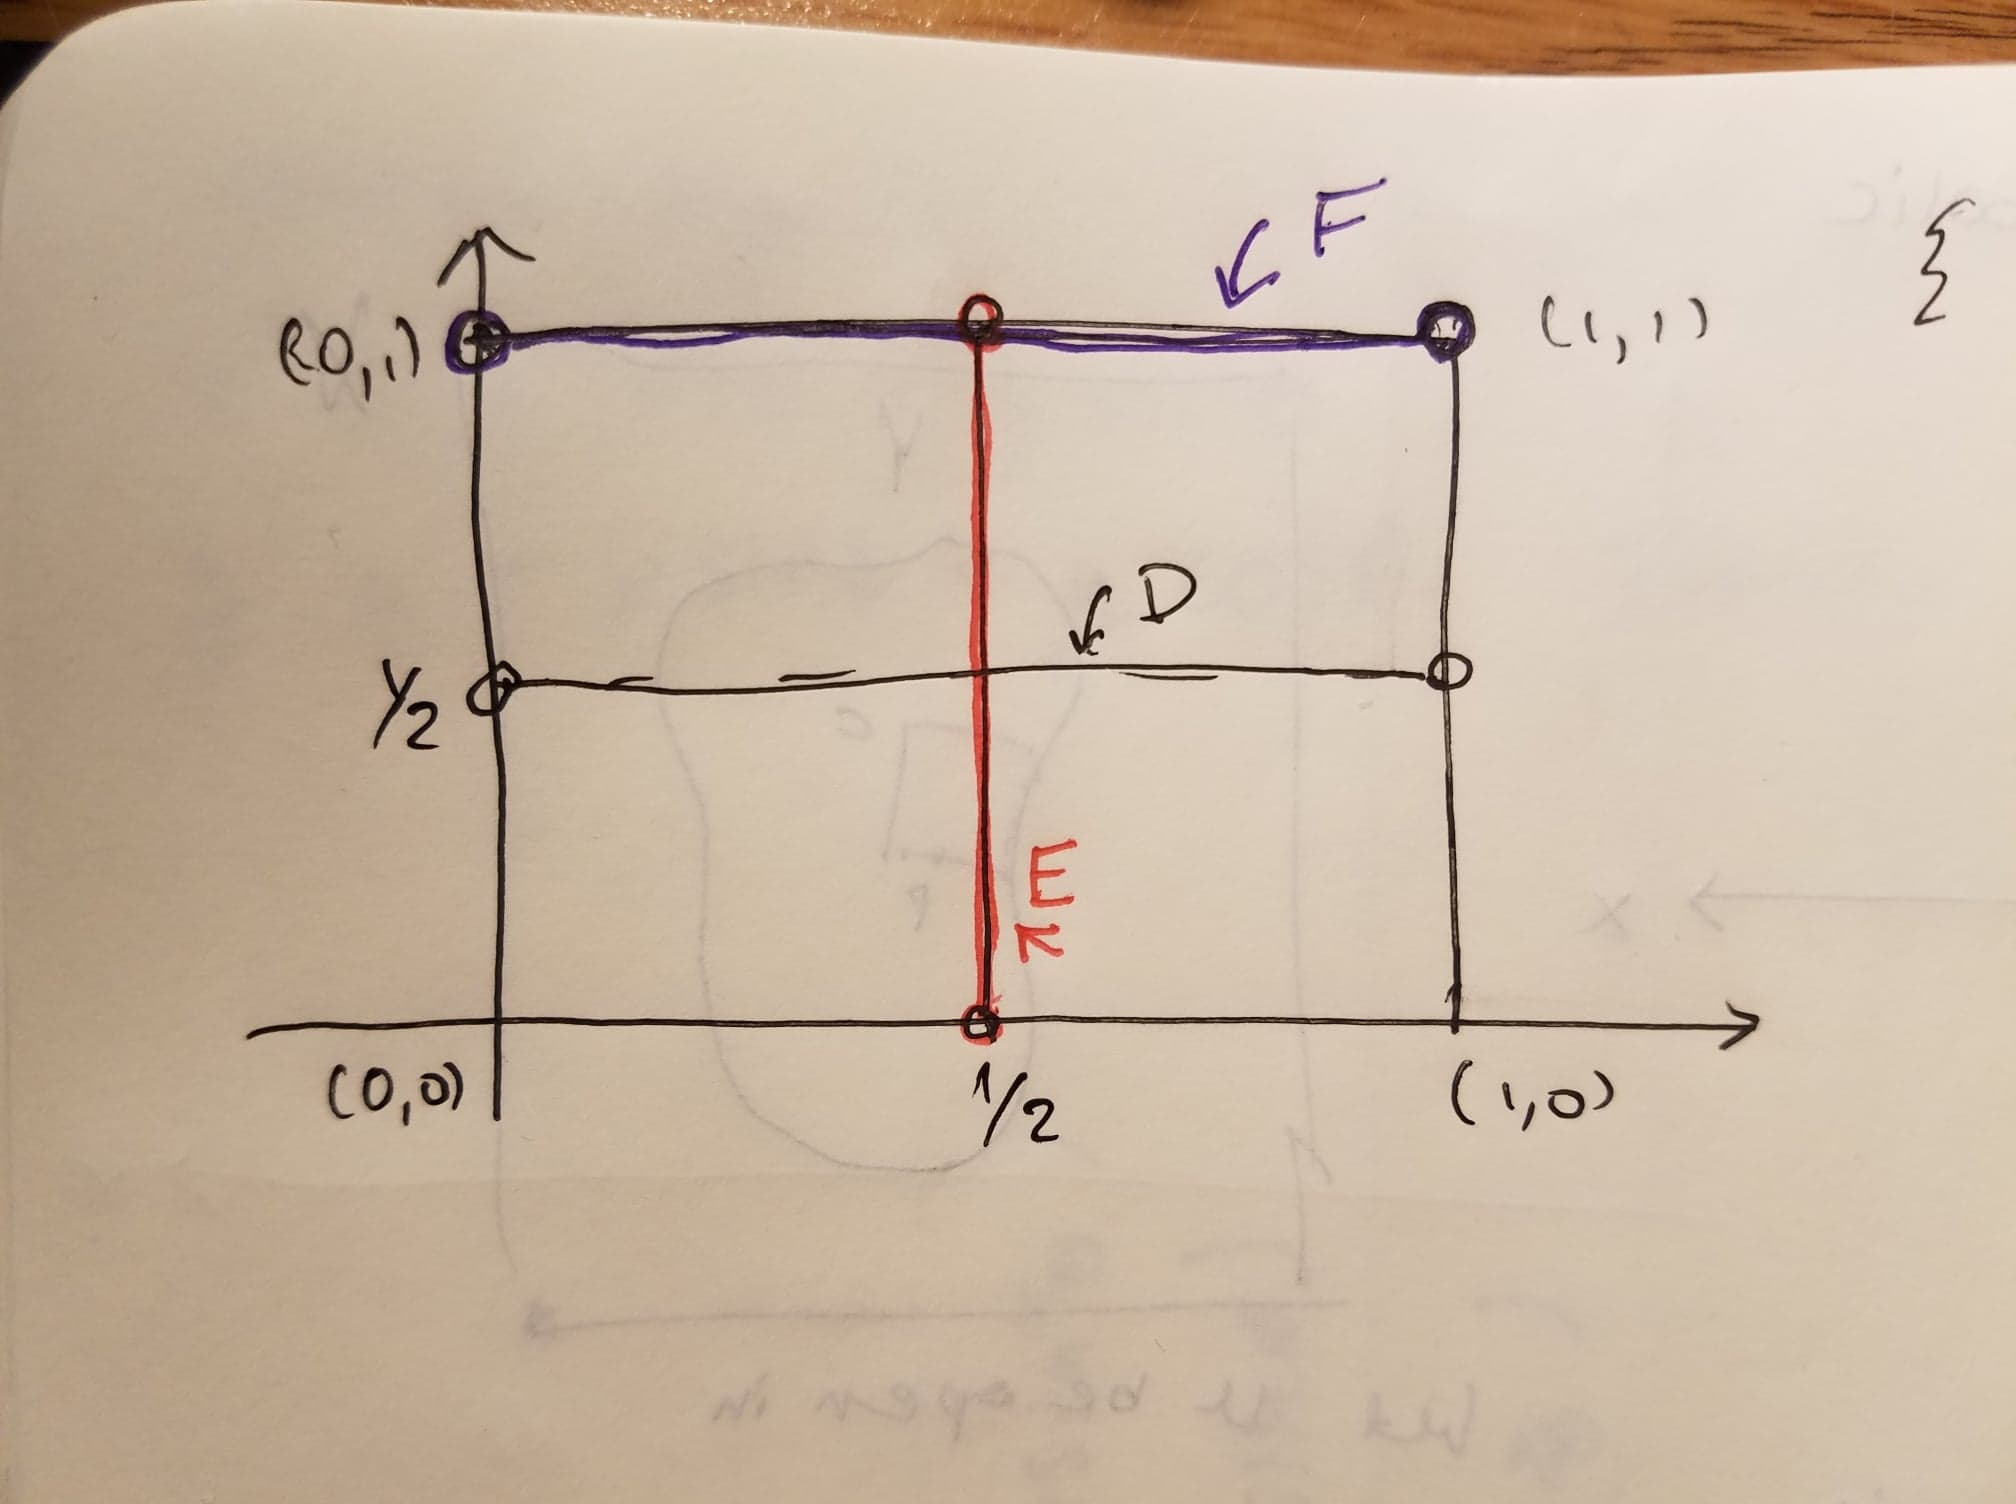
\includegraphics[width = \textwidth]{figures_theorems_sect_4/exercise_4_31.jpg}
\end{figure}

\begin{exercise}[Exercise 4.32]
    Verify that the collection of basic open sets
    above satisfies the conditions of Theorem 4.3, thus confirming that
    this collection is a basis for a topology.
\end{exercise}

\begin{solution}
First observe that the first condition of Theorem 4.3 is satisfied,
since for any $(p, q) \in X \times Y$ there exist open sets $U \in X$
and $V \in Y$ such that $p \in U$ and $q \in V$. Thus there exists a
basic open set $U \times V$ such that $(p, q) \in U \times V$, which
shows that each point of $X \times Y$ is in some basic open set. \\
\\
Now suppose $U, V$ are basic open sets. Then $U = A \times B$ and $V =
C \times D$ for some open sets $A, C \in \mathscr{T}_X$ and $B, D \in
\mathscr{T}_Y$. Let $p \in U \cap V = (A \cap C) \times (B \cap D)$.
Then observe that $(A \cap C) \in \mathscr{T}_X$ and $(B \cap D) \in
\mathscr{T}_Y$. Since the basis consists of the product of all open
sets in $X$ and all open sets in $Y$, we see that $(A \cap C) \times
(B \cap D)$ must be a basic open set. Thus we have a basis element $W
= (A \cap C) \times (B \cap D)$
such that $p \in W \subset U \cap V$, which satisfies the second part
of Theorem 4.3. Thus the proposed collection is in fact a basis for
the topology.
\end{solution}

\begin{exercise}[Exercise 4.33]
    Draw examples of basic and arbitrary open sets
in $\mathbb{R}^2 = \mathbb{R} \times \mathbb{R}$ using the standard
topology on $\mathbb{R}$. Find (i) an open set in $\mathbb{R} \times
\mathbb{R}$ that is not the product of open sets, and (ii) a closed
set in $\mathbb{R} \times \mathbb{R}$ that is not the product of
closed sets.
\end{exercise}

\begin{figure}[h!]
    \centering
    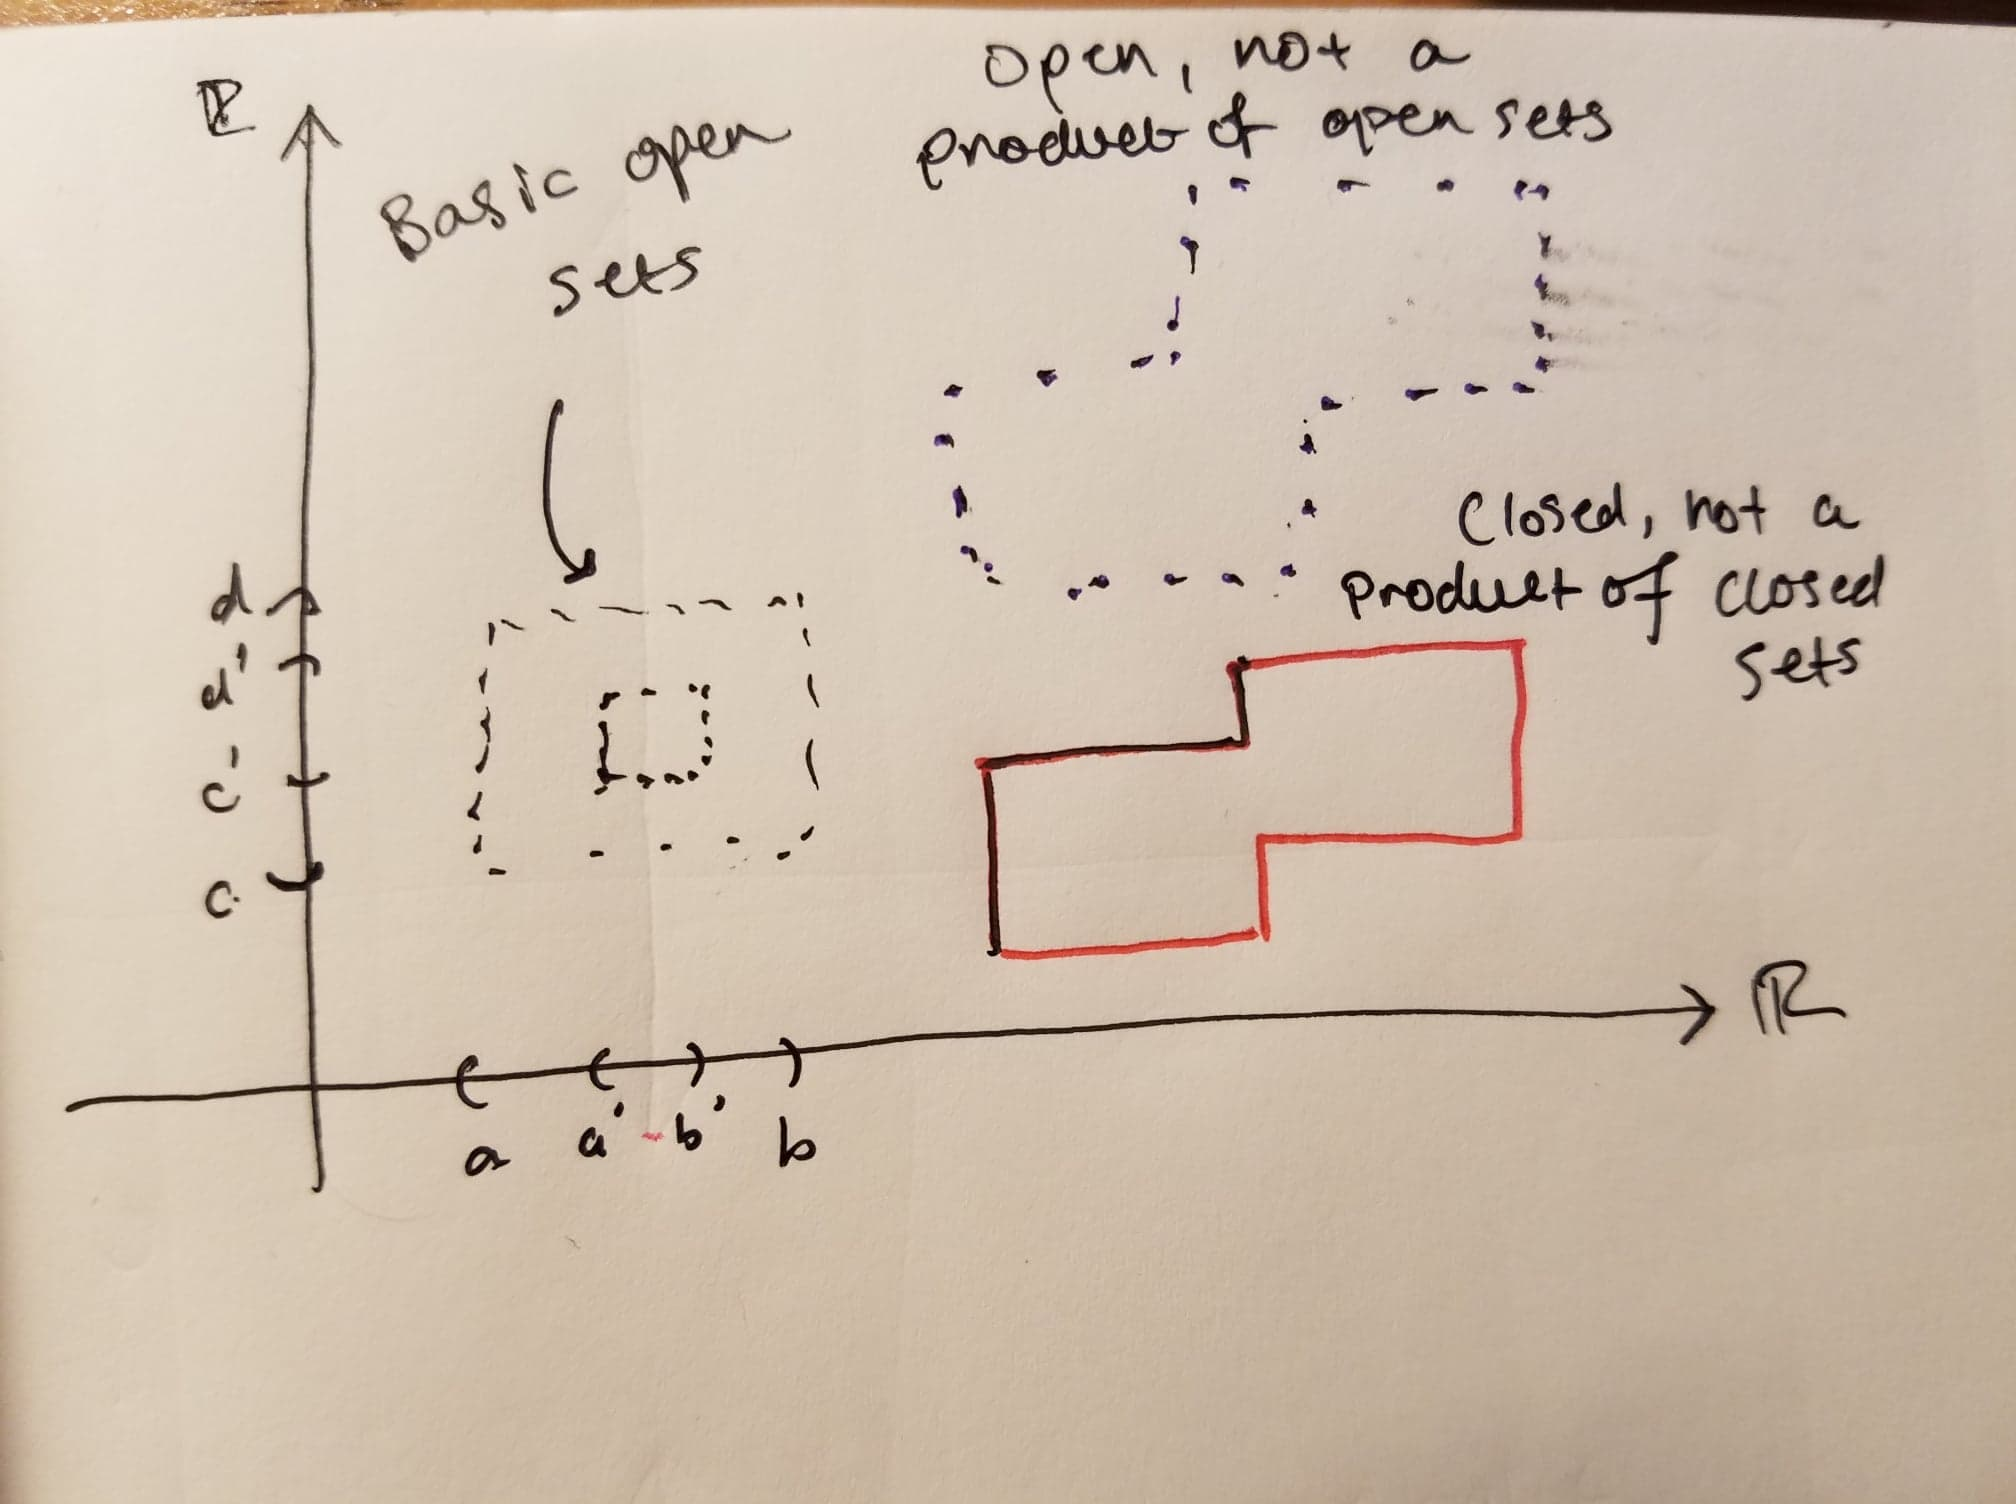
\includegraphics[width = 0.7\textwidth]{figures_theorems_sect_4/exercise_4_33.jpg}
\end{figure}

\begin{exercise}[Exercise 4.34]
    Is the product of closed sets closed?
\end{exercise}

\begin{solution}
    Yes.
Let $p \in \overline{U}$ and $q \in \overline{V}$. Then for every open set $U_p$ 
containing $p$ and $V_q$ containing $q$, we'll have that $U_p \cap U \ne \emptyset$
and $V_q \cap V \ne \emptyset$. Therefore we see that $(U_p \times U_q) \cap (U \times V)
\ne \emptyset$, meaning that $(p, q) \in \overline{U \times V}.$ Thus we have 
that $\overline{U} \times \overline{V} \subset \overline{U \times V}$.
\\
\\
Now suppose $(p, q) \in \overline{U \times V}$. Then every basic open
set of the form $U'\times V'$ containing $(p, q)$ intersects $U
\times V$. In other words, for every open set $U' \in
\mathscr{T}_X$ containing $p$, then $U' \cap U \ne \emptyset$. Similarly, for every
open $V' \in \mathscr{T}_Y$ containing $q$, $V' \cap V \ne \emptyset$
Thus we must have that $p \in \overline{U}$ and $q \in \overline{V}$, 
so that $(p, q) \in \overline{U} \times \overline{V}$, which implies
that $\overline{U \times V} \subset \overline{U} \times \overline{V}$.
\\
\\
Since $\overline{U \times V} \subset \overline{U} \times \overline{V}$
and $\overline{U} \times \overline{V} 
\subset \overline{U \times V}$, we have that $\overline{U \times V}
= \overline{U} \times \overline{V}$.  Thus if $U, V$ are closed,
$\overline{U} = U$ and $\overline{V} = V$, so $U \times V =
\overline{U \times V}.$ So the product of closed sets is in fact closed. 
\end{solution}

\begin{exercise}[Exercise 4.35]
    Show that the product topology $X \times Y$ is
the same as the topology generated by the subbasis of inverse images
of open sets under the projection functions, that is the subbasis is
$\{\pi^{-1}_{X}(U) | U \text{ is open in } X\} \cup \{\pi^{-1}_{Y} (V)
| V \text{ is open in } Y\}.$ 
\end{exercise}

\begin{solution}
Let $U$ be open. Then for $p \in U$, there exists a basic open 
set $W \in \mathscr{T}_\text{prod}$, the product topology, such that 
\[
   p \in W \subset U. 
\]
Observe that $W = W_x \times W_y$ where $W_x \in \mathscr{T}_x$ and $W_y \in
\mathscr{T}_y$. Note also that
\[
   W = W_x \times W_y = (W_x \times Y) \cap (X \times W_y).
\]
Let $\mathscr{S}$ be the set of inverse images of open sets under the
projection functions. Then we also know that $\pi_X^{-1}(W_x) = W_x
\times Y$, while
$\pi_X^{-1}(W_y) = X \times W_y$, which are in $\mathscr{S}$.
We can then state that 
\[
    W = \pi_X^{-1}(W_x) \cap \pi_Y^{-1}(W_y).
\] 
Therefore, we see that 
\[
    p \in \pi_X^{-1}(W_x) \cap \pi_Y^{-1}(W_y) \subset W.  
\]
Since for each $V \in \mathscr{S}$ we have that 
$V \in \mathscr{T}_\text{prod}$, (1) $\mathscr{S} \subset
\mathscr{T}_\text{prod}$ and (2) for any open set $U$ and 
point $p \in W$ there exists elements $\pi_X^{-1}(W_x), \pi_X^{-1}(W_y)
\in \mathscr{S}$ such that 
$p \in \pi_X^{-1}(W_x) \cap \pi_Y^{-1}(W_y) \subset U$, 
we have by Theorem 4.14 that 
$\mathscr{S}$ is a subbasis of the product topology, as desired.
\end{solution}

\begin{exercise}[Exercise 4.36]
    Using the standard topology on $\mathbb{R}$, is
the product topology $\mathbb{R}\times\mathbb{R}$ the same as the
standard topology on $\mathbb{R}^2$?
\end{exercise}

\begin{solution}
Consider
$B(p, R)$, a disk of radius $R$ centered at $p = (p_x, p_y)$,
which is an open set in $\mathbb{R}_\text{std}$. 
\\
\\
Observe that for each $q = (q_x, q_y) \in B(p, R)$, we can construct a
set $U_q = (q_x - \epsilon, q_x + \epsilon)$
containing $q_x$ if 
\begin{gather*}
    p_x - R < q_x - \epsilon \quad q_x + \epsilon < p_x + R
\end{gather*}
and similarly we can for the set $V_q = (q_y - \delta, q_y + \delta)$ containing $q_y$ if
\begin{gather*}
    p_y - R < q_y - \delta \quad q_y + \epsilon < p_y + R.
\end{gather*} 
Therefore, $q \in U \times V \subset B(p, R)$. Since for each $q \in
B(p, R)$ we can find an open $W_p = U_q \times V_q$ such that $p \in
W_q \subset B(p, R)$, we see that 
\[
   \bigcup\limits_{q \in B(p, R)} W_q =  B(p, R).
\]
Thus we see that the product topology is a subset of the standard
topology on $\mathbb{R}$.
Now consider a basic open set $W = U \times V$ 
in the product topology on $\mathbb{R}\times \mathbb{R}$.
Thus $U =(a, b)$ and $(c, d)$, where $a, b, c, d$ may or may not be
finite.
\\
\\
Observe that for any $p = (p_x, p_y) \in U \times V$, we can contain
it in a ball $B(p, \epsilon)$ where 

\[
    \epsilon <\min\{\min\{b-p_x,p_x-a\}, \min\{c-p_y, p_y - c\}\}.
\]
Therefore, we see that for any $p \in U \times V$ there exists an open
ball $B(p, \epsilon)$ such that $p \in B(p, \epsilon) \subset U \times
V$. Hence 
\[
    \bigcup\limits_{p \in U \times V}B(p, \epsilon_p) = U \times V 
\]
so that the standard topology is a subset of the product topology. 
Since we show the converse, we must have that the standard topology is
equivalent to the product topology on $\mathbb{R}$.
\end{solution}

\begin{exercise}[Exercise 4.37]
    A basis for the product topology on $\prod\limits_{\alpha \in \lambda}
X_\alpha$ is the collection of all sets of the form
$\prod\limits_{\alpha \in \lambda}U_\alpha$ where $U_\alpha$ is open
in $X_\alpha$ for each $\alpha$ and $U_\alpha = X_\alpha$ for all but
finitely many $\alpha$.
\end{exercise}

\begin{solution}
Consider an open set $U$ in the product topology $\mathscr{T}_\text{prod}$. Then for each $p \in
U$, there exists a subbasic open set in $\mathscr{S}$ such that 
\[
   p \in \bigcap\limits_{i = 1}^n \pi^{-1}_{\alpha_i}(U_{\alpha_i}) 
   \subset U
\]
Now consider the family of sets described in the problem, and call
this set $\mathscr{T}_\text{prod}'$. 
Observe that we can write 
\[
    \bigcap\limits_{i = 1}^n \pi^{-1}_{\alpha_i}(U_{\alpha_i})
    = \dots \times U_{\alpha_1} \times \dots \times U_{\alpha_n} \times \dots
    = \prod\limits_{\alpha \in \lambda} U_{\alpha}
\] 
where $U_\alpha  = X_\alpha$ for all $\alpha \in
\lambda\textbackslash\{\alpha_1, \alpha_2, \dots, \alpha_n\}$ 
and $U_{\alpha_1}, U_{\alpha_2}, \dots U_{\alpha_n}$ are all
restricted open sets in the spaces $X_{\alpha_1}, X_{\alpha_2}, \dots
X_{\alpha_n}$, respectively. Thus $\mathscr{S} \subset
\mathscr{T}_\text{prod}'$.
\begin{align}
  p \in \prod\limits_{\alpha \in \lambda}U_\alpha \subset U.  
\end{align}
Now observe that for any $V \in \mathscr{T}_\text{prod}'$, $V =
\prod\limits_{\alpha \in \lambda}U_\alpha$ where $U_\alpha$ is open
in $X_\alpha$ for each $\alpha$ and $U_\alpha = X_\alpha$ for all but
finitely many $\alpha$,
\[
    V = \prod\limits_{\alpha \in \lambda} U_{\alpha}
    = \dots \times U_{\alpha_1} \times \dots \times U_{\alpha_n} \times \dots
    = \bigcap\limits_{i = 1}^n \pi^{-1}_{\alpha_i}(U_{\alpha_i})
\]
Thus we see that $\mathscr{T}_\text{prod}' \subset
\mathscr{S}$, so that these two collections of sets generate the same
topology: namely, the product topology. More specifically, we see that
(1) $\mathscr{T}_\text{prod}' \subset \mathscr{T}_\text{prod}$ and 
(2) equation (1) satisfies Theorem 4.3, which proves
that $\mathscr{T}_\text{prod}$ forms a basis for the product topology,
as desired.
\end{solution}

\begin{exercise}[Exercise 4.38]
    Let $\mathscr{T}$ be the topology on $2^X$
with basis generated by the subbasis $\mathscr{S}$. 
\begin{itemize}
    \item[1.] Every basic open set in $2^X$ is both open and closed.

    \item[2.] Show that if a collection of subbasic open sets of $2^X$ has the
    property that every point of $2^X$ lies in at least one of those
    subbasic open sets, then there are two subbasic open sets in that
    collection such that every point of $2^X$ lies in one of those two
    subbasic open sets.

    \item[3.] Show that if a collection of basic open sets of $2^X$ has the
    property that every point of $2^X$ lies in at least one of those basic
    open sets, then there are a finite number of basic open sets in that
    collection such that every point of $2^X$ lies in one of those basic
    sets. 
\end{itemize}
\end{exercise}

\begin{solution}
    \begin{itemize}
        \item[1.]Consider an arbitrary basic open set $U$ in the product topology of
        $2^X$. Then observe that $U$ is of the form 
        \[
           U = \{f \in 2^X : f(a_1) = \delta_1, f(a_2)= \delta_2, \dots, f(a_n)= \delta_n\} 
        \]
        where $a_1, \dots, a_n \in A$ and $\delta_1, \delta_2, \dots, \delta_n
        \in \{0, 1\}$. Then observe that 
        \[
            U^c = \{f \in 2^X: f(a_1) = |\delta_1-1|, f(a_2)= |\delta_2-1|, \dots, f(a_n)= |\delta_n-1|\}
        \]
        Since $U$ is open, $U^c$ is closed. However, $U^c$ is still of the form
        of basic open set, which means that $U$ is closed. Therefore, every
        basic open set in $2^X$ is open and closed.
    
        \item[2.] Let our subbasic open cover be $\{U_{\alpha}\}_{\alpha \in
        \lambda}$ where $U_\alpha \in \mathscr{T}$ for all $\alpha \in
        \lambda.$ Now suppose there aren't two subbasic open sets such
        that every point of $2^X$ lies in one or the other. Then observe
        that this is not a cover of $2^X$ since, if a point of $2^X$ lies
        in one set $U$, then it does not lie in $U^c$. Thus in this case
        it would not even be a cover.
    
     
        \item[3.] Let $\{U_\alpha\}_{\alpha \in \lambda}$ be our cover as
        previously defined. Fix $p \in 2^X$, and observe it lives in some
        subbasic set 
        \[
          U = \{f \in 2^X : f(a_1) = \delta_1, f(a_2) = \delta_2, \dots, f(a_n) = \delta_n \}. 
        \]
        Observe that every point of $x$ either lies in this set, or its
        coordinate values $f(a_1), f(a_2), \dots, f(a_n)$ differ in at least one
        coordinate from the restriction offered by $U$. Since every
        coordinate can have at most 2 different values, we see that there
        are $2^n$ different ways that the coordinate values $f(a_1),
        f(a_2), \dots , f(a_n)$ could differ from the restriction offered
        in $U$. Thus we can have at most $2^n + 1$ basic open sets
        which contain all the points in $X$, which means that there are at
        most a finite number of basic open sets that cover every point of $2^X$. 
    \end{itemize}
\end{solution}

\begin{exercise}[Exercise 4.39]
    In the product space $2^{\mathbb{R}}$, what is the closure of the set
$Z$ consisting of all elements of $2^\mathbb{R}$ that are 0 on
every rational coordinate, but may be 0 or 1 on any irrational
coordinate? Equivalently, thinking of $2^{\mathbb{R}}$ as subsets
of $\mathbb{R}$, what is the closure of the set $Z$ consisting of
all subsets of $\mathbb{R}$ that do not contain any rational? 
\end{exercise}

\begin{solution}
Observe that 
\[
    Z^c = \bigcup_{n \in \mathbb{N}}^{\infty} \{f : {2}^{\mathbb{R}} | f(a_1) = f(a_2) = \cdots = f(a_n) = 0, a_1, a_2, \dots, a_n \in \mathbb{Q}\}
\]
where $a_1, a_2, \dots, a_n$ are distinct but arbitrarily chosen of
$\mathbb{Q}$. Note that this is an uncountable union of open sets,
since we are only making a finite number of restrictions on the
coordinates. Therefore $Z$ must be closed, so $\overline{Z} = Z$.
\end{solution}

\begin{exercise}[Exercise 4.40]
    Find a subset $A$ of $2^\mathbb{R}$ and a limit
point $x$ of $A$ such that
no sequence in $A$ converges to $x$. For an ever greater challenge,
determine whether you can find such an example if $A$ is countable.
\end{exercise}

\begin{solution}
Observe that the point $p \in 2^{\mathbb{R}}$ such that 
\begin{gather*}
    p(a) = 1 \quad \forall a \in \{\pi + q : q \in \mathbb{Q}\}\\
    p(a) = 0 \quad \forall a \in \mathbb{R} - \{\pi + q : q \in \mathbb{Q}\}
\end{gather*} 
is a limit point of $Z$, the set consisting of
all elements of $2^\mathbb{R}$ that are 0 on every rational coordinate
and 0 or 1 on all others.
(Note: $\pi$ was chosen randomly. We could have done it with any other
irrational. All we want is a point such that it's $x$-th coordinate is
1 for a countable number of irrational $x$. We know $\mathbb{Q}$ is
countable, so adding $\pi$ to every element of this set generates a
countable set of irrationals, which is how we want to design our point.)
\\
\\
Any open set containing $p$ must be of the form 
\[
    \{
        f \in 2^\mathbb{R} | f(\pi + q_1) = f(\pi + q_2) = \cdots = f(\pi + q_n) = 1, q_1, q_2, \
        \dots, q_n \in \mathbb{Q}  
    \}
\]
and hence will intersect $Z$.
\\
\\
By Theorem 3.30, if there exists a sequence
of elements of $Z$ which converge to $p$ then $p \in \overline{Z}.$
But in 4.39 we saw $\overline{Z} = Z$, and clearly $p \not\in Z$.
Hence $p \not\in \overline{Z}$, so there is no sequence of elements of
$Z$ which converge to $p$. 
\end{solution}

\begin{exercise}[Exercise 4.41]
    Let $\mathbb{R}^\omega$ be the countable product of copies of
    $\mathbb{R}$. So every point in $\mathbb{R}^\omega$ is a sequence
    $(x_1, x_2, x_3, \dots).$ Let $A \subset \mathbb{R}^\omega$ be the set
    consisting of all points with only positive coordinates. Show that in
    the product topology, $\mathbf{0} = (0, 0, 0, \dots)$ is a limit point
    of the set $A$, and there is a sequence of points in $A$ converging to
    $\mathbf{0}$. Then show that in the box topology, $\mathbf{0} = (0, 0,
    0, \dots)$ is a limit point of the set $A$, but there is no sequence
    of points in $A$ converging to $\mathbf{0}$.
\end{exercise}

\begin{solution}
Let $U$ be an open set containing $\mathbf{0}$. Suppose $\mathbf{0}$ is in 
the basic open set $B$ of the product topology so that 
$B = \Pi_{\alpha \in \omega} U_\alpha$ where $U_\alpha$ is open 
in $\mathbb{R}$, and $U_\alpha = \mathbb{R}$ for all but finitely many 
$\alpha$. Then for each $\alpha \in \omega$ corresponding to $U_\alpha 
\ne \mathbb{R}$, the open set must contain $\mathbf{0}$, and hence it must contain
positive points of $\mathbb{R}$. Since the rest of the $U_\alpha$'s 
such that $U_\alpha = \mathbb{R}$ obviously contain positive coordinates of 
$\mathbb{R}$, we see that the basic open set, and hence the set $U - \{\mathbf{0}\}$, 
must have a
nonempty intersection with $A$. Therefore $\mathbf{0}$ is a limit point of 
$A$ in the product topology.
\\
\\
I claim that the sequence $(\frac{1}{n}, \frac{1}{n}, \dots )$
is a sequence which converges to $\mathbf{0}$ in the product topology. 
Observe that we can contain $\mathbf{0}$ in a
basic open set $B$, where again $B = \Pi_{\alpha \in \omega} U_\alpha$ and $U_\alpha$ is open 
in $\mathbb{R}$ while $U_\alpha = \mathbb{R}$ for all but finitely many 
$\alpha$. Thus for each $U_\alpha \ne \mathbb{R}$, let $n_\alpha \in \mathbb
{N}$ be such that $\frac{1}{n_\alpha} \in U_\alpha$. Now let 
$$
n = \min\left\{n_\alpha \Big| \frac{1}{n_\alpha} \in U_\alpha\right\}.
$$
Then for $i > n$, we see that $(\frac{1}{i}, \frac{1}{i}, \dots ) \in B$. 
Thus every open set about $\mathbf{0}$ will contain points of the sequence, which 
shows that this sequence converges to $\mathbf{0}$ in the product topology.
\\
\\
Now we'll show that there is no sequence which converges to $\mathbf{0}$ 
in the box topology. Suppose for the sake of contradiction that there is a sequence 
of points 
$$
\begin{matrix}
    (a_{11} & a_{12} & a_{13} & \dots)\\
    (a_{21} & a_{22} & a_{23} & \dots) \\
    (a_{31} & a_{32} & a_{33} & \dots) 
  \end{matrix} $$
which converge to $\mathbf{0}$. Then observe that 
we can construct an open set about $\mathbf{0}$ in the box topology
as follows. Let $(a_1, a_2)$ contain $0$ but exclude $(a_{11})$. 
Let $(a_3, a_4)$ contain $\mathbf{0}$ but exclude $(a_{22})$. If 
we continue in this fashion, we'll construct an open set in the box topology
$$
(a_1, a_2) \times (a_3, a_4) \times \dots
$$
which all contain $\mathbf{0}$ but exclude every point of the proposed sequence.
The fact that we can create this open set containing $\mathbf{0}$ but no element 
of the sequence contradicts our claim, which shows that no sequence in the box 
topology can converge to $\mathbf{0}$.
\end{solution}

\begin{exercise}[Exercise 4.42]
Show that the set $2^\mathbb{N}$ in the box topology is a discrete
space, whereas the set $2^\mathbb{N}$ in the product topology has no
isolated points. 
\end{exercise}

\begin{solution}
Observe that we can think of an open set here under the box topology as a 
a set of points where we are allowed to make an infinite number of
restrictions on each coordinate. With this perspective, it is then
clear that every point is a basic open set, since every point $p$ has
a restriction on every single coordinate. Since every point is open,
we have that all subsets of $2^\mathbb{N}$ are open, which implies
that the set is a discrete space under the box topology.
\\
\\
Consider any basic open set in $2^\mathbb{N}$ under the product topology:
\[
   U = \{f \in 2^\mathbb{N} : f(a_1) = \delta_1, \dots , f(a_n) = \delta_n\} \quad \delta_1, \dots , \delta_n \in \{0, 1\}
\] 
Observe that the set contains the point
\[
    p = (\dots, \hspace{-2mm} \overbrace{\delta_{1}}^{\text{$f(a_1)$}}\hspace{-2mm}, \dots, \hspace{-2mm} \overbrace{\delta_{2}}^{\text{$f(a_2)$}}\hspace{-2mm}, \dots,\hspace{0.5mm} \overbrace{\delta_{n}}^{\text{$f(a_n)$}}\hspace{0.5mm}, \dots, \hspace{-6mm} \overbrace{\delta_{n +1}}^{\text{unrestricted by $U$}}\hspace{-6mm}, \dots)
\]
where $\delta_{n+1} \in \{0, 1\}$. But $U$ also contains another point $p'$ such that 
\[
    p' = (\dots, \hspace{-2mm} \overbrace{\delta_{1}}^{\text{$f(a_1)$}}\hspace{-2mm}, \dots, \hspace{-2mm} \overbrace{\delta_{2}}^{\text{$f(a_2)$}}\hspace{-2mm}, \dots,\hspace{0.5mm} \overbrace{\delta_{n}}^{\text{$f(a_n)$}}\hspace{0.5mm}, \dots, \hspace{-4mm} \overbrace{1 - \delta_{n +1}}^{\text{unrestricted by $U$}}\hspace{-4mm}, \dots).
\]
Thus no basic open set in $2^\mathbb{N}$ in the product topology
contains a single element. Hence, there are no isolated points.
\end{solution}

\end{document}
